\begin{figure}[h]
    \centering
    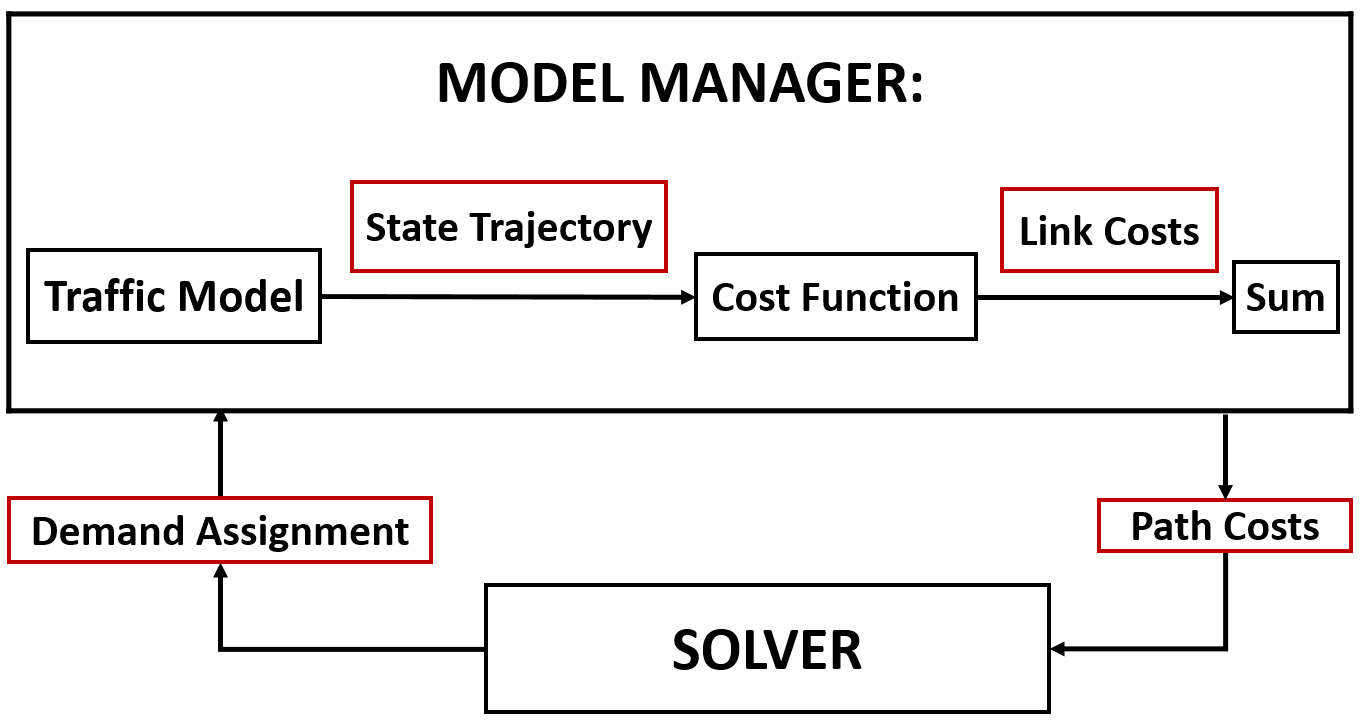
\includegraphics[width=\linewidth]{figs/Software_Block_Diagram.PNG}
    \caption{Software framework has a modular design, which allows to easily extend the framework.}
    \label{fig:Block_Diagram}
\end{figure}

Using the unified VI formulation and the generic iteration shown in \ref{fig:iteartion}, we designed a modular and extensible software framework to solve traffic assignment problems, including static and dynamic traffic problems. Figure~\ref{fig:Block_Diagram} show that the software framework has two main modules: the Model Manager and the Solver modules. The Demand Assignment and Path Costs components are wrappers for demand assignment $h$, and for path travel costs respectively $c$.

The Model Manager has three components that correspond function $F$: the Traffic Model, Cost Function and Sum components. The software framework currently include three traffic models: ST, MN, and CTM, which all integrate in the framework via the Traffic Model component. These are implemented using the Beats simulator, which is a  The State Trajectory module is a wrapper for link states (e.g: flow per link), and the Link Cost module is a wrapper for the travel cost per link (e.g experienced travel time on a link). The Model Manager's role is to translate an assignment $h$, specified as a sequence of demand per path by the Demand Assignment module, into the corresponding path costs, represented as a sequence of cost per path.

The Solver module serves as an interface to plug in solution algorithms for DTA. The SOLVER works in a loop in which it generates candidate demand assignments, and expects to be given the corresponding network path costs. This loop continues until an equilibrium demand assignment is reached. The Solver interface allows to incorporate different DTA solution algorithm. We included three solver algorithms: the MSA, the FW, and the EPM, which can be applied depending on the $F$ function properties. 

The advantage of our modular software framework is that it can be easily extended to address different traffic assignment problems by including new traffic models, cost functions, and solver algorithms. For example, the framework has a travel time based cost function. A user can add an energy or emission based cost function. For problems, such as simulation-based DTA problems, where the traffic model is tightly coupled with the cost function evaluation, a user can integrate implementation of the $F$ function without having to write the Traffic model, Cost Function and Sum modules . The complete documentation on software framework, with installations instructions can be found at \cite{ta_solver}